\documentclass[a4paper,10pt]{scrartcl}

\usepackage[dvips,pdftex]{graphicx}
\usepackage[latin1]{inputenc}
\usepackage[ngerman]{babel}
\usepackage[T1]{fontenc}
\usepackage[automark]{scrpage2}
\pagestyle{scrheadings}
\usepackage{graphicx}
\usepackage{color}
\usepackage{alltt}
\usepackage{listings}



%\definecolor{mygreen}{rgb}{0,0.6,0}
\definecolor{mygray}{rgb}{0.5,0.5,0.5}
%\definecolor{mymauve}{rgb}{0.58,0,0.82}

\lstset{
%  backgroundcolor=\color{white},   % choose the background color; you must add \usepackage{color} or \usepackage{xcolor}
  basicstyle=\footnotesize,        % the size of the fonts that are used for the code
  breakatwhitespace=false,         % sets if automatic breaks should only happen at whitespace
  breaklines=true,                 % sets automatic line breaking
  captionpos=b,                    % sets the caption-position to bottom
%  commentstyle=\color{mygreen},    % comment style
  deletekeywords={...},            % if you want to delete keywords from the given language
  escapeinside={\%*}{*)},          % if you want to add LaTeX within your code
  extendedchars=true,              % lets you use non-ASCII characters; for 8-bits encodings only, does not work with UTF-8
%  frame=single,                    % adds a frame around the code
  keepspaces=true,                 % keeps spaces in text, useful for keeping indentation of code (possibly needs columns=flexible)
%  keywordstyle=\color{blue},       % keyword style
  language=VHDL,                   % the language of the code
%  morekeywords={*,...},            % if you want to add more keywords to the set
  numbers=left,                    % where to put the line-numbers; possible values are (none, left, right)
  numbersep=5pt,                   % how far the line-numbers are from the code
  numberstyle=\tiny\color{mygray}, % the style that is used for the line-numbers
%  rulecolor=\color{black},         % if not set, the frame-color may be changed on line-breaks within not-black text (e.g. comments (green here))
  showspaces=false,                % show spaces everywhere adding particular underscores; it overrides 'showstringspaces'
  showstringspaces=false,          % underline spaces within strings only
  showtabs=false,                  % show tabs within strings adding particular underscores
  stepnumber=2,                    % the step between two line-numbers. If it's 1, each line will be numbered
%  stringstyle=\color{mymauve},     % string literal style
  tabsize=2,                       % sets default tabsize to 2 spaces
  title=\lstname                   % show the filename of files included with \lstinputlisting; also try caption instead of title
}





\begin{document}

% Title Page
\begin{titlepage}
\begin{center}
\begin{Large}

\sffamily \vspace*{\fill}{Institut f\"ur Computertechnik\\
Labor integrierte Schaltungen\\
384.088\\}
\vfill { Labor\"ubung Sommersemester 2005\\}
\vspace{10mm}{\textbf{Beispiel 7: Tempomat}\\}
\vspace{10mm}{Betreuer: Herr Nachtnebel}\\
\today\\
\end{Large}
\vfill

% use packages: array
\begin{tabular}{llll}
\textbf{Matr. Nr} & \textbf{Vor- und Zuname} & \textbf{E-mail} & \textbf{Note} \\
0527734 & Klotzner Robert & e0527734@student.tuwien.ac.at &  \\
0726765 & R. Christian Tessarek & christian.tessarek@tuwien.ac.at &
\end{tabular}

\end{center}
\end{titlepage}



\pagebreak
\tableofcontents
\pagebreak


\section{Aufgabenstellung}
\label{sec:aufgabe}

TODO: BLALBA Beschreiben Sie die Aufgabenstellung
The FPGA development board's features, especially the rotary knob and the LCD display, should be used to mimic a speed control system. 
A micropocessor should be implemented on top of the FPGA, running an assembly program which implements the required speed control application. 

Inputs are the rotary knob sensor readings (2 logic signals) and the rotary knob push button logical signal, which should be used as reset. 
The outputs are connected to the LCD display and show the current setpoint value of the speed control. 

The speed should not increase/decrease with more than 5km/h/sec to ensure a soft acceleration/deceleration. 

The microcontroller should be implemented using a Von-Neumann architecture and should be able to process one assembly instruction per clock cycle. 


\section{Blockschaltbild}
\label{sec:block}

% Zeichnen Sie das Blockschaltbild Ihrer Realisierung.

\begin{figure}[ht]
	\centering
\noindent\makebox[\textwidth]{
	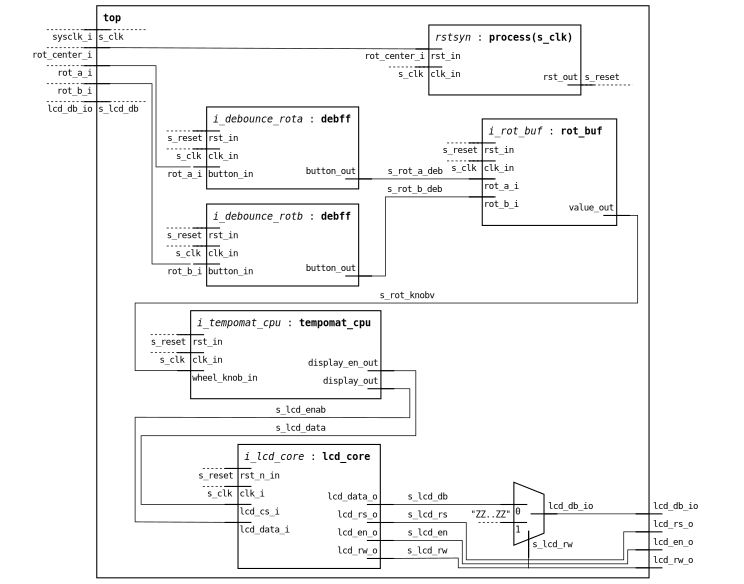
\includegraphics[keepaspectratio,width=\paperwidth]{diagram01}
}
	\caption{Blockschaltbild}
	\label{fig:block}
\end{figure}

\clearpage


\subsection{Beschreibung der Schaltung}
\label{sec:schaltung}

TODO: blabla...was tu ma da?


\subsection{Befehlscodierung}
\label{sec:bef_cod}

% Beschreibung des Befehlssatzes mit der gew\"ahlten Codierung

TODO: evtl allgemeines blabla


\noindent\texttt{ 0  =>  IN\_C}

Beschreibung blabla

\noindent\texttt{ 1  =>  OUTL\_C}

Beschreibung blabla

\noindent\texttt{ 2  =>  OUTH\_C}

Beschreibung blabla

\noindent\texttt{ 3  =>  OUTCR\_C}

Beschreibung blabla

\noindent\texttt{ 4  =>  LDI\_C}

Beschreibung blabla

\noindent\texttt{ 5  =>  INC\_C}

Beschreibung blabla

\noindent\texttt{ 6  =>  DEC\_C}

Beschreibung blabla

\noindent\texttt{ 7  =>  STR\_C}

Beschreibung blabla

\noindent\texttt{ 8  =>  LDR\_C}

Beschreibung blabla

\noindent\texttt{ 9  =>  CMP\_C}

Beschreibung blabla

\noindent\texttt{10  =>  JC\_C}

Beschreibung blabla

\noindent\texttt{11  =>  JZ\_C}

Beschreibung blabla

\noindent\texttt{12  =>  JMP\_C}

Beschreibung blabla

\noindent\texttt{13  =>  WAIT\_C}

Beschreibung blabla



\section{Assemblerprogramm}
\label{sec:ass_prog}

% F"ugen Sie das Assemblerprogramm ein und beschreiben Sie es.

TODO: beschreibungs-blabla laalaa


\begin{alltt}\footnotesize
 0: \textbf{LDI }
 1: \textit{0}
 2: \textbf{STR}
 3: \textbf{OUTCR}
 4: \textbf{OUTH}
 5: \textbf{OUTL}
 6: \textbf{IN}
 7: \textbf{CMP}
 8: \textbf{LDR}
 9: \textbf{JZ }
10: \textit{17}
11: \textbf{JC }
12: \textit{16}
13: \textbf{DEC}
14: \textbf{JMP }
15: \textit{17}
16: \textbf{INC}
17: \textbf{WAIT }
18: \textit{200}
19: \textbf{JMP }
20: \textit{2}
\end{alltt}



\section{VHDL Source-Code}
\label{sec:vhdl}

% F\"ugen Sie den VHDL Code ein und beschreiben Sie ihn.

TODO: vhdl source code blabla lala

\subsection{comp\_pack}
blabla sdfdf

\lstinputlisting[title={comp\_pack.vhd}]{../vhd/comp_pack.vhd}

\subsection{debff}
This modules contains a flip-flop-based debouncer used for knob button input debouncing. 

\lstinputlisting[title={debff\_.vhd}]{../vhd/debff_.vhd}

\lstinputlisting[title={debff\_rtl.vhd}]{../vhd/debff_rtl.vhd}

\subsection{rot\_buf}
This modules decodes the inputs of the two rotary knob sensors to the tempomat speed set value. 

\lstinputlisting[title={rot\_buf\_.vhd}]{../vhd/rot_buf_.vhd}

\lstinputlisting[title={rot\_buf\_rtl.vhd}]{../vhd/rot_buf_rtl.vhd}

\subsection{tempomat\_cpu}
This modules represents the CPU executing the above described assembly program. 

\lstinputlisting[title={tempomat\_cpu\_.vhd}]{../vhd/tempomat_cpu_.vhd}

\lstinputlisting[title={tempomat\_cpu\_rtl.vhd}]{../vhd/tempomat_cpu_rtl.vhd}

\subsection{top}
This modules is the top entity. 

\lstinputlisting[title={top\_.vhd}]{../vhd/top_.vhd}

\lstinputlisting[title={top\_struc.vhd}]{../vhd/top_struc.vhd}



\subsection{Testbench}
\label{sec:bench}

% Beschreiben Sie die Testbench und f"ugen Sie das Simulationsresultat ein.

The testbench \texttt{tb\_top} module is connected with its inputs to the outputs of the \texttt{top} module and vice-versa, its outputs with the inputs of the \texttt{top} entity. 
It first initializes the inputs of the \texttt{top} module, thereby testing the reset functionality as well. 
Then, turning the knob up, and then, down again is simulated with two for-loop. 
Important is that the counter does not overflow when reaching the maximum value of 255 and that it doesn't ``underflow'' at 0.

Because it is not possible to directly access signals inside a module without creating an extra port and because the output of the \texttt{lcd\_core} module is not really (easily) tracable/ well-documented, both the \texttt{debff} debouncer module and the \texttt{rot\_buf} module are tested with their own respective testbench modules, \texttt{tb\_debff} and \texttt{tb\_rot\_buf}. 


\lstinputlisting[title={tb\_top.vhd}]{../sim/tb_top.vhd}

\lstinputlisting[title={tb\_debff.vhd}]{../sim/tb_debff.vhd}

\lstinputlisting[title={tb\_rot\_buf.vhd}]{../sim/tb_rot_buf.vhd}


\subsubsection{Simulation Results}

The \texttt{tb\_rot\_buf} module uses assertions to ensure the module behaves correctly in the aforementioned circumstances; no assertion errors where triggered running the simulation. 

The \texttt{tb\_debff} module's simulation results are shown in Fig.\ \ref{fig:debff01}; it can be seen that after $600\mathrm{us}$ of a signal being stable, it is passed on to the output. 

The \texttt{tb\_top} module uses similar stimuli as the \texttt{tb\_rot\_buf} module to test the correct behavior of the CPU and execution of the assembly program. 

\begin{figure}[ht]
	\centering
%\noindent\makebox[\textwidth]{
	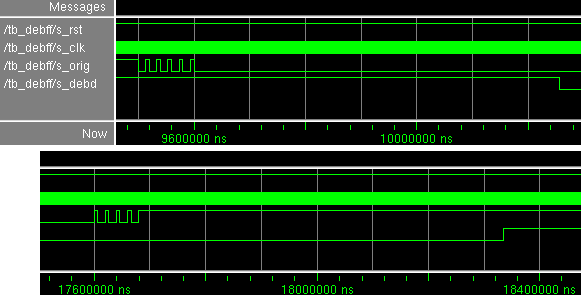
\includegraphics[keepaspectratio,width=\textwidth]{debff01}
%}
	\caption{Simulation Details -- Debouncer Module}
	\label{fig:debff01}
\end{figure}


\end{document}
